\chapter{CMB mapmaking in practice}

As we have mentioned, CMB telescope do not take pictures, as the signal-to-noise ratio of each picture would be too low.  Instead they scan the sky keeping track of the power they collect and where they are pointed.  The process of reassembling the image of the sky is called mapmaking.


\begin{figure}
  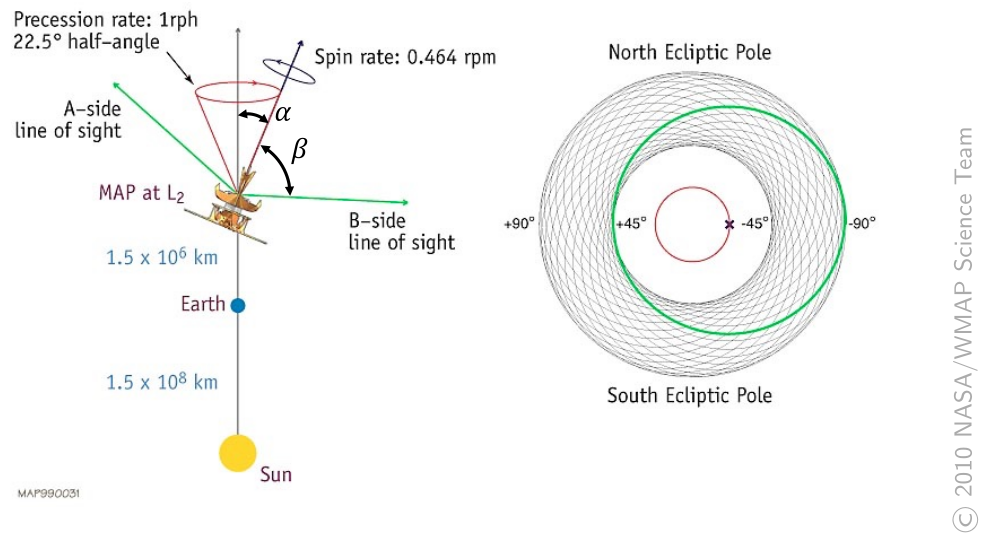
\includegraphics[width=\linewidth]{figs/CMB_mapmaking/wmap_scan.png}
  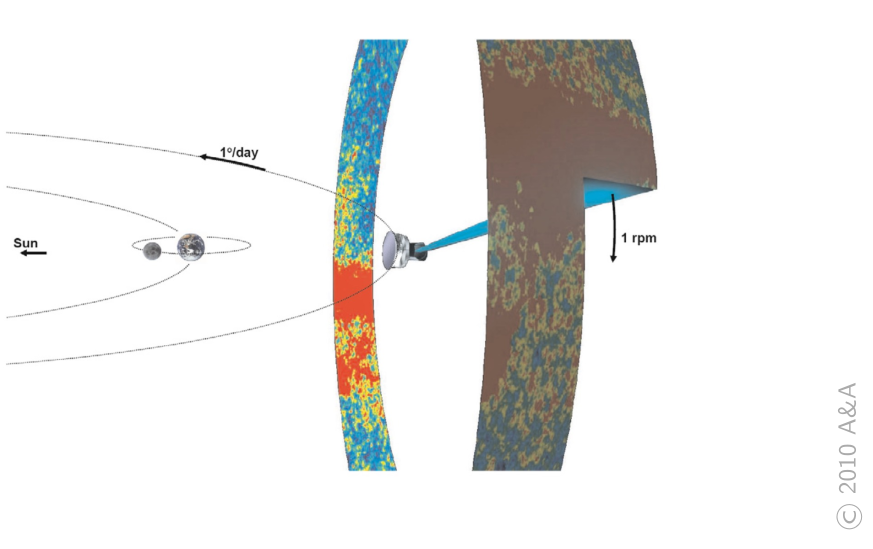
\includegraphics[width=\linewidth]{figs/CMB_mapmaking/planck_scan.png}
  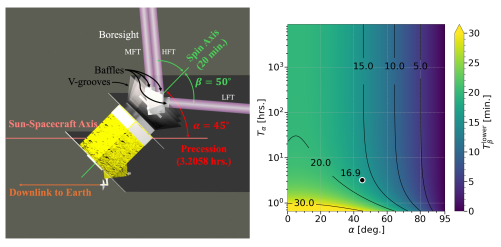
\includegraphics[width=\linewidth]{figs/CMB_mapmaking/litebird_scan.png}
  \caption{Scan strategies for space-based missions.  WMAP and LiteBIRD do fast precession scans of a doughnut shape that gradually shift as the spacecraft orbits the Sun.  Planck does thin rings (thinner than depicted) that similarly shift as the spacecraft orbits, but is only strongly cross linked at the poles.\citep{2025arXiv250303176T}}
\end{figure}


\begin{figure}
    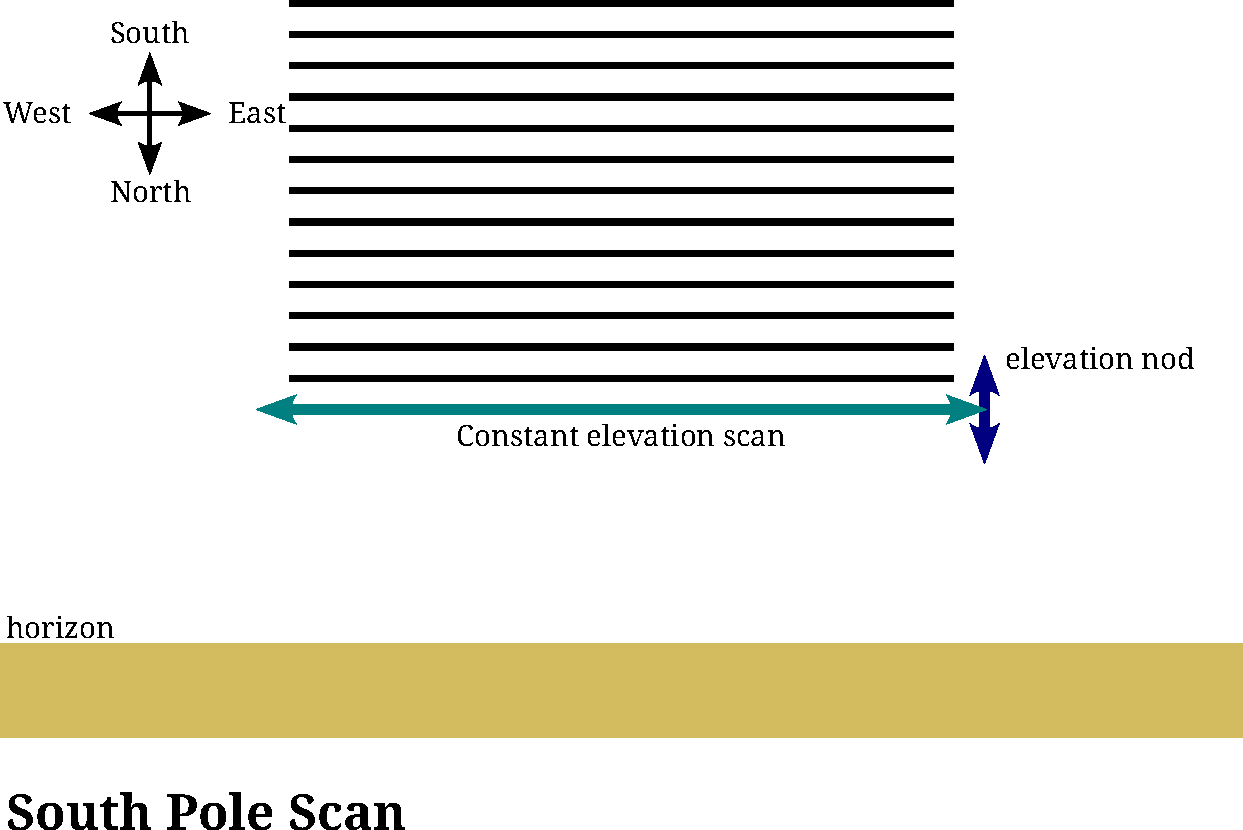
\includegraphics[width=0.5\linewidth]{figs/CMB_mapmaking/SPT_scan.pdf}
    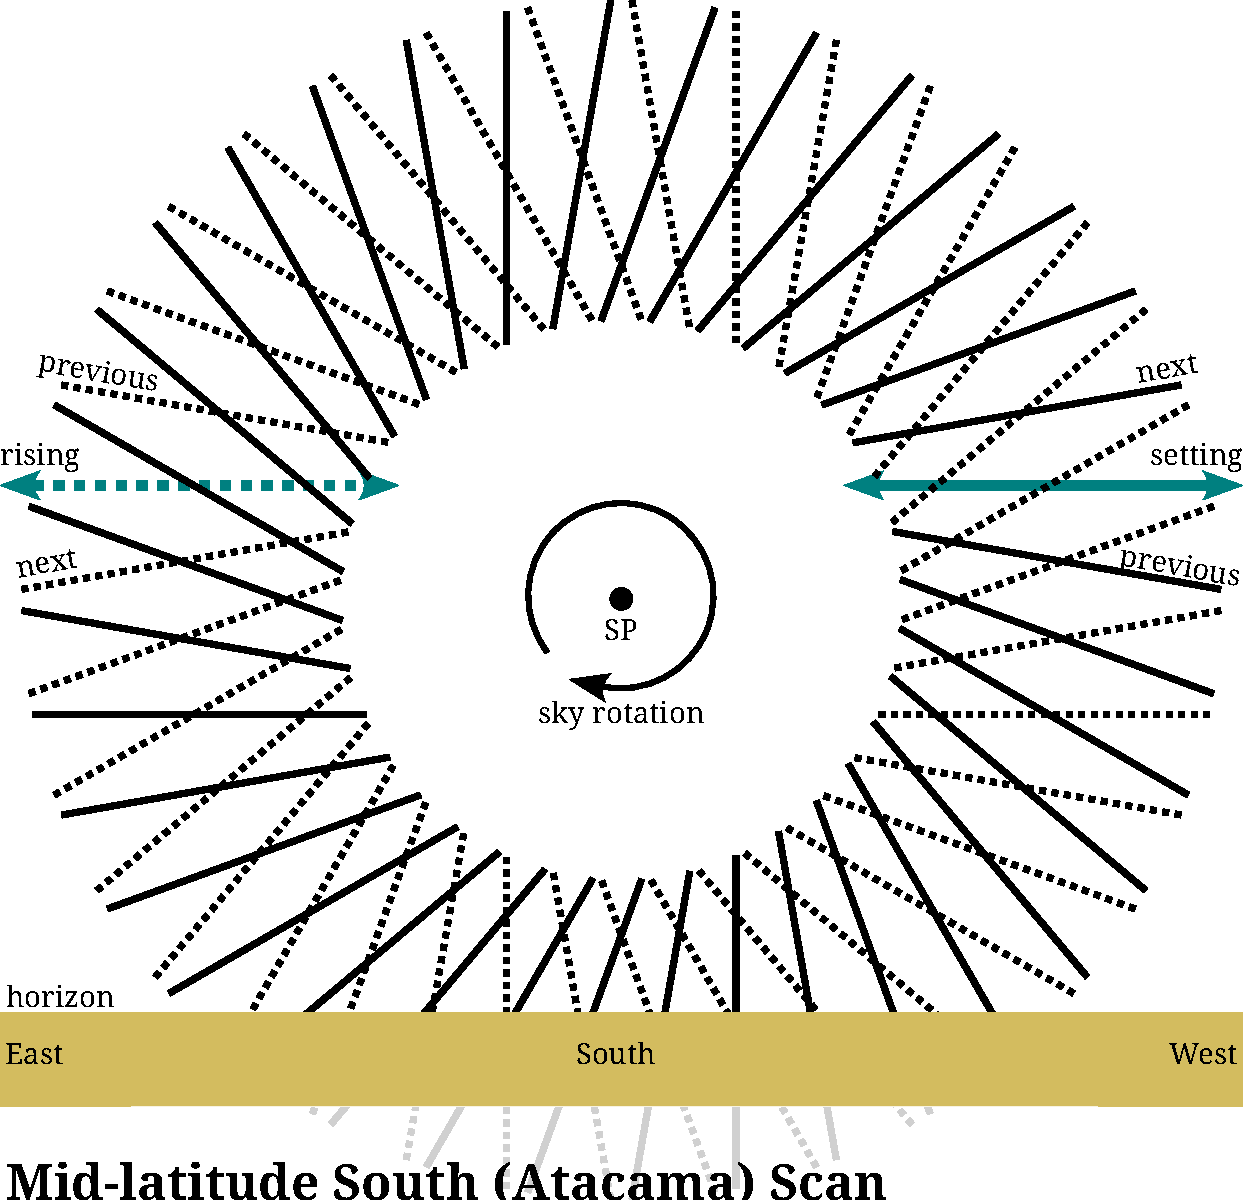
\includegraphics[width=0.5\linewidth]{figs/CMB_mapmaking/ACT-SO_scan.pdf}
    \caption{Ground-based CMB scannning strategies.}
\end{figure}


\section{Time-ordered data and calibration}

\begin{equation}
  d(t_i) = \int d\Omega R(t_i,\theta,\phi) s(\theta,\phi) + n(t_i)
\end{equation}
where $s$ is the sky signal.

Planck satellite calibration on dipole and orbital changes to the dipole.

band pass

gain calibration

detector time constants; time constant deconvolution

deglitching

data cuts

gap filling


\section{Mapmaking}

We approximate the time-ordered data (TOD) as 
\begin{equation}
  d_i = P_{ip}s_p + n_i \qquad \mbox{or} \qquad d = Ps + n
\end{equation}
The $P$ matrix has number of time sample columns and number of map pixels rows.  It is extremely large, and not square.  The pencil beam approximation is that $P_{ip} = 1$ if the detector points at map pixel $p$ and zero otherwise, only one entry per row.  This makes it very sparse.  The pencil beam assumption is that we are observing a beam-convolved map with perfect resolution rather than what we are actually doing, which is observing an unconvolved sky with a coarser beam resolution.

For any candidate map solution, we could write an estimate of the noise as $n' = d-Ps'$.  Then if the timestream noise has a covariance matrix $N = \langle n n^\dag \rangle$ (more on this in a minute) we can construct the following $\chi^2$ statistic
\begin{equation}
  \chi^2(s') = (d-Ps')^\dag N^{-1} (d-Ps') 
\end{equation}

We can see what linear operation on the data produces a candidate map, 
\begin{equation}
  s' = Wd
\end{equation}
and the minimize $\chi^2$, or maximize a Gaussian likelihood based on it, to find $W$ under the constrain that the map is unbiased.  The calculus and algebra is doable and yields $W = (P^\dag N^{-1}P)^{-1} P^\dag N^{-1}$, so that we have a formal solution to the mapmaking equation as

\begin{equation}
\bar s = (P^\dag N^{-1}P)^{-1} P^\dag N^{-1}d \label{eqn:mapmaking}
\end{equation}

This is essentially a weighted average of the time ordered data $d$.  This solution is known in statistics as the Generalized Least Squares\index{Generalized Least Squares solution} (GLS) solution, and in the CMB community as Maximum Likelihood Mapmaking\index{Maximum likelihood mapmaking}.  

We can show that the solution is unbiased by substituting in the data $d = Ps +n$ and taking the ensemble average.
\begin{equation}
\langle \bar s \rangle = (P^\dag N^{-1}P)^{-1} P^\dag N^{-1} \langle Ps + n \rangle
\end{equation}
For a particular realization of the of the CMB sky, only the noise is a random variable, and the mean of the noise is zero, $\langle n \rangle = 0$.  So we find
\begin{equation}
\langle \bar s \rangle = (P^\dag N^{-1}P)^{-1} P^\dag N^{-1} P s = s
\end{equation}
When we cancel $P^\dag N^{-1} P$ with its inverse, we found $\langle \bar s \rangle = s$, so $\bar s$ is unbiased, giving the right sky on average.  Note if we assume the wrong covariance matrix for the timestream noise, say $M$ instead of $N$, we would still get an unbiased map:
\begin{equation}
\langle \bar s \rangle = (P^\dag M^{-1}P)^{-1} P^\dag M^{-1} P s = s.
\end{equation}
Thus we are robust to our inaccurate knowledge of the noise covariance.  We will get a suboptimal map, but not an biased one.

The noise in the timestream tends to be red on long time scales and white on short time scales and is fairly stationary.  Noise may be correlated between pairs of detectors, especially if two detectors are in the same horn or on the same readout line within an optics tube. Thus a reasonable model for the noise covariance matric is diagonal in the frequency domain, describable by a power spectrum, and block diagonal among detectors,
\begin{equation}
  \langle n(\omega)_k n(\omega)_{k'}^*  \rangle = 2\pi P^N_{kk'}(\omega) \delta(\omega - \omega') 
\end{equation}
for frequency $f = \omega/2\pi$ and detector pair $kk'$  for timestream harmonics
\begin{equation}
n_k(t) = \int df\, n(f = \omega/2\pi) \exp(2\pi i ft) = \int \frac{d\omega}{2\pi}\, n(\omega) \exp(i \omega t)
\end{equation}
This we know how to handle from the descriptions in Chapter \ref{ch:correlations}, substituting $t \rightarrow x$ and $\omega \rightarrow k$.

\paragraph{Conjugate gradient descent.}  Now we turn to how in the world we can actually solve the mapmaking Equation (\ref{eqn:mapmaking}).  The matrix $P^\dag N^{-1} P$ has size of the number of pixels on a side, far too large to invert directly at model resolutions.  However, because it is composed of sparse and diagonal pieces, we are able to compute the matrix multiplications of them.  So we rearrange the equation to the standardized linear form $Ax = b$,
\begin{equation}
  (P^\dag N^{-1}P) \bar s = P^\dag N^{-1}d.
\end{equation}
This equation contains several operations on map-like or TOD-like objects ($\mathsf{s}$ or $\mathsf{d}$). Each is computationally tractable.  Often, we do not literally need to write the matrices out to memory, but we can write a routine to compute the result of the product:
\begin{itemize}
\item $N^{-1} \mathsf{d}$: we compute the time-frequency fourier transform for the set of detectors, then invert $N(\omega)$ frequency by frequency, and multiply times the coefficients of the detector set.  When all frequencies are done, we transform the detector harmonics back to the time domain.  The input and output are both timestreams.
\item $P \mathsf{s}$: from the maplike object, we generate a synthetic timestream, simulating the pointing of the telescope to read out the pixel values at the appropriate positions of the detectors for every time sample.  The input is a map and the output is a timestream.
\item $P^\dag \mathsf{d}$: this is the opposite operation.  Here we accumulate in each map pixel the sum of all time sample values that fall within it.  The input is a timestream and the output is a map.
\end{itemize}

Returning to the linear form $Ax = b$, both side of the equation describe map-sized objects, and we can efficiently compute all the operations to compute $b$ and multiply map $x$ by $A$.  Matrix $A$ is square, positive definite, symmetric, and invertible, but we are unable to store or invert it.


How do we build the noise model?  If we have a guess of the map, we can compute and estimate for the noise as
\begin{equation}
  \bar n = d - P \bar s
\end{equation}
and estimate its power spectrum as we know how to do.
Since the signal is low, we make the first pass with the approximation that $\bar n = d$, then make a refined noise model based on the map estimate. Two-pass mapmaking is usually suffficient, but sometimes more passes are necessary.

map noise covariance
 
computing a single row

If the noise is white, the proper mapmaking is very simple:
\begin{equation}
  \bar s =  (P^\dag P)^{-1} P^\dag d
\end{equation}
Bin the data up into pixels and normalize by the number of samples per pixel ($N_\textrm{obs}$).


An alternative is filter and bin map making.  A prewhitening filter fourier $M^{-1}$ suppresses the red portion of the noise, then we proceed with the simplified map making.
\begin{equation}
  \bar{\bar s} =  (P^\dag P)^{-1} P^\dag M^{-1} d
\end{equation}
The uncorrected $M$ leaves a bias in the map that is reflected in the power spectrum:
\begin{equation}
  \langle \mathcal{C}^\textrm{obs}_b \rangle = \sum_l \mathcal{W}_{bl} (F^M_l C_l)
\end{equation}
This transfer function from the filtering $F^M_l$ can be estimated by a Monte Carlo process.  Thus while filter and bin mapmaking has a very rapid mapmaking process, the simulations, which are about as costly as CG steps, are a significant computational burden.

Gain fluctuations is a model error,
\begin{equation}
  d = g(t) Ps + n
\end{equation}
also adds a transfer function even to ML mapmaking \cite{Naess and Louis}.


\section{Noise in the map}

\paragraph{Anistropic uncorrelated noise.}  Where a telescope looks more, there is less noise.
We can add the next level of realism by modulating the noise covariance proportional to the number of observation samples a telescope measured in each pixel.  This gives the noise covariance in the pixel basis this form:
\begin{equation}
N_{pp'} =  \sigma^2_p \delta_{pp'}= \frac{\sigma^2}{\Delta\Omega_p N_\textrm{obs}(p)}  \delta_{pp'}
\end{equation}

This model for the noise covariance is diagonal in pixel space but non-diagonal in harmonic space.  We can still compute the effective pseudo-power spectrum of that noise (more on this below) finding that it is
\begin{equation}
\langle \tilde N_l \rangle = \frac{\sigma^2}{4\pi} \sum_p  \left(\frac{1}{N_\textrm{obs}(p)} \right)^2.
\end{equation}
The noise is still white, but it is not uniform or isotropic.

\paragraph{Translation invariant, anisotropic 2d noise.}  This noise is homogeneous but not isotropic.  This type of noise uses the flat sky approximation to assign power to 2d Fourier harmonics, but different harmonics get different variances. This is written as
\begin{equation}
N_{\textrm{2d tr.\ inv.},\mathbf{ll'}} = \left\langle n(\mathbf l) n(\mathbf l')^* \right\rangle = N(\mathbf{l}) \delta_\mathbf{ll'}.
\end{equation}
This is diagonal in the harmonics, so while larger to describe than an isotropic $N_l$, it is still tractable to store and invert.  The power in the noise is often anisotropically distributed, as in Figure \ref{fig:act_DR6_noise}, with certain scan or other directions getting more noise variance.

This type of noise is statistically invariant under translations in the plane of the sky, but not rotations.  The flat sky approximation breaks down on scales larger than $\sim 10^\circ$, so this method cannot treat large sky areas.

\paragraph{Realistic noise.}
\begin{figure}
  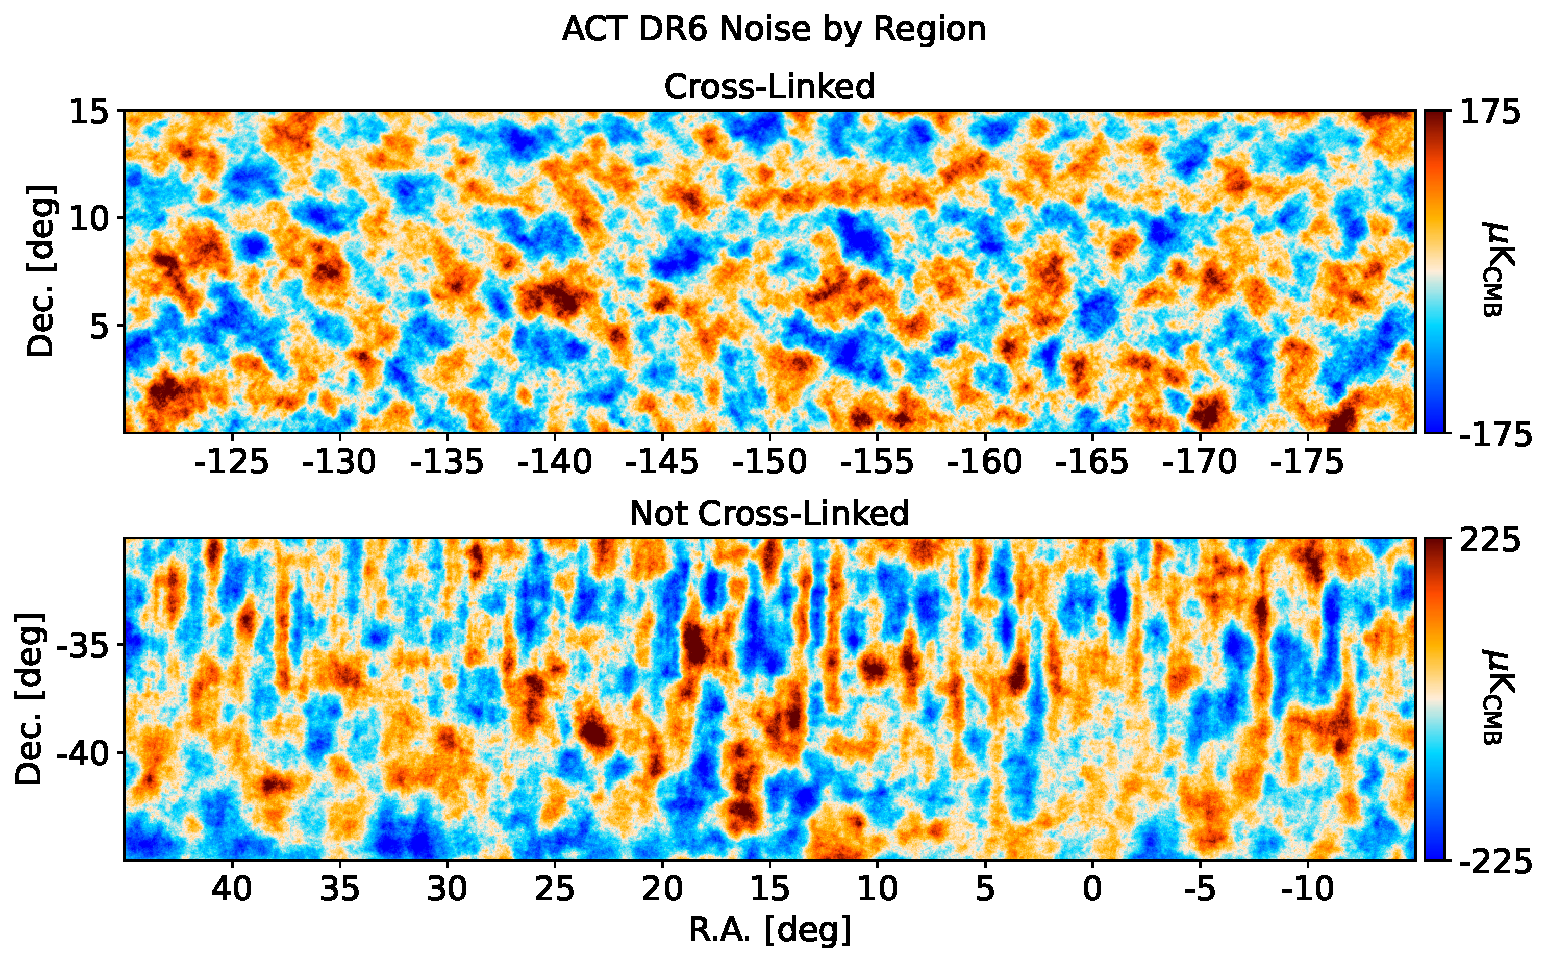
\includegraphics[height=5.2cm]{figs/CMB/Atkins2024pa5_f090_set0_map_T.pdf}\hfill
  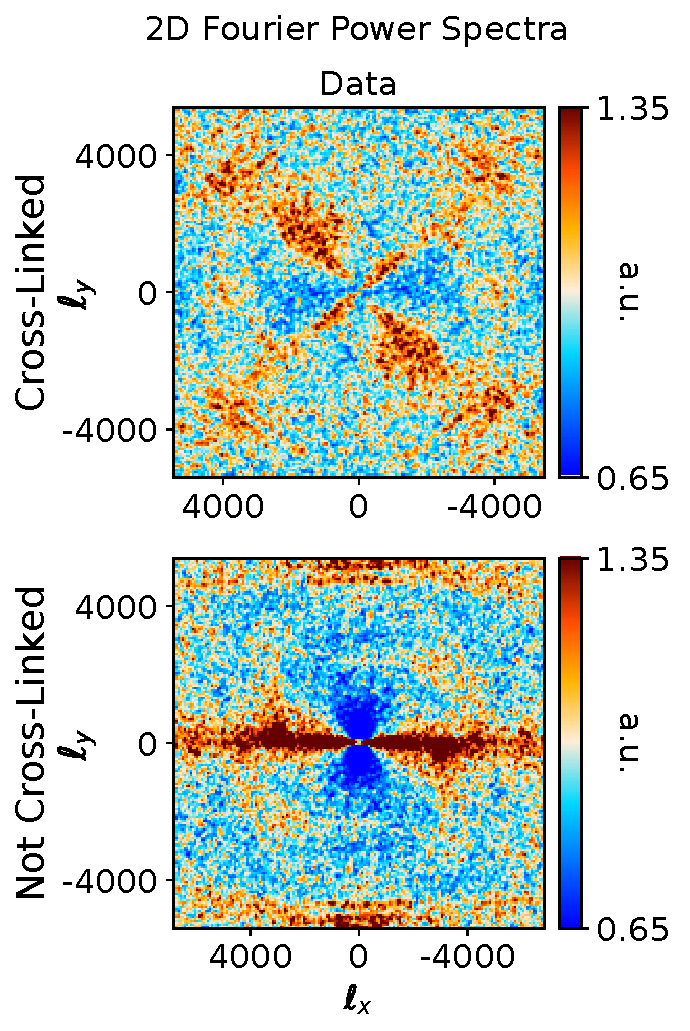
\includegraphics[height=5.2cm]{figs/CMB/Atkins2024_pa5_f090_set0_2d_T_sims.pdf}
  \caption{Noise-only map computed from a difference of ACT Data Release 6 (DR6) \citep[from][]{2025JCAP...05..015A}.  Left are the noise maps for two regions of the sky, above with good cross-linking, diagonal-left and diagonal-right scans that are not very visible.  The second with nearly-parallel, vertical scans and bad cross linking.  Right are the 2d flat-sky-approximation Fourier components, displayed as amplitude-squared.  The orientation of the scans is more visible here.  Above shows the complicated and anistropic noise behavior.  Below, the strong vertical striping is caused by noise modes with $l_y \approx 0$.} \label{fig:act_DR6_noise}
\end{figure}

In  Figure \ref{fig:act_DR6_noise}, we see a visualization of the map noise in the ACT data.  This is made from taking the difference of map splits, labeled $A$ and $B$, where maps are made from two distinct but equivalent halves of the data:
\begin{equation}
  d^A = T + n^A  \qquad d^B = T + n^B.
\end{equation}
A coadded map is 
\begin{equation}
  \frac{1}{2} ( d^A  + d^B ) = T +  \frac{1}{2} (n^A + n^B),
\end{equation}
while the difference map is
\begin{equation}
  \frac{1}{2} ( d^A - d^B ) =  \frac{1}{2} (n^A - n^B)
\end{equation}
Because $n^A$ and $n^B$ are independent random variables, the sum and the difference have the same variance.  The temperature signal cancels in the difference map, so it is a realization of pure noise.  Although the noise in the difference map is not literally the same as the coadd map, for gaussian noise, it is drawn from the same distribution.

We can test any particular noise model to see if the difference map could have been drawn from it.  Using a different split yields a different noise map, but it is correlated to other noise maps and to the coadded map with signal becuase, ultimately, they derive from the same total data.

A few types of models attempt to capture more of the salient features of the complicated noise of the type in Figure \ref{fig:act_DR6_noise}, which has directional, anisotropic features that vary across the sky.  In the tiled \textit{constant correlation} noise model \citep{2020JCAP...12..046N}, 

\begin{equation}
N^{-1} = W^{-1/2} N_\textrm{2d tr.\ inv.}^{-1} W^{-1/2}
\end{equation}
where a pixel-diagonal weighting matrix
\begin{equation}
  W^{-1/2}_{pp'} = N_\textrm{obs}(p) ^{1/2} w_\textrm{tile}(p) \delta_{pp'}
\end{equation}
modulates the Fourier-harmonic-diagonal noise matrix
$ N_\textrm{2d tr.\ inv.}$ describing the local power.
By breaking up the sky into localized tiles, idea is that we can use the local flat-sky approximation to characterize the local anisotropic power in the noise, which normally would be translation invariant, but the weighting matrix spatially adjusts the the variance in response to the number of oberservations and allows us with $w_\textrm{}(p)$ to manage the transition to another tile where the local power is distributed differently.  This helps to handle changes in scan directions across the sky.  Unfortunately, it cannot encode correlations larger than the tile size, which is limited by the flat sky approximation.


Tiling is just one multi-scale approach, where the properties on different scales and different locations are handled separately by using a series of tractable operations.  Another is a \textit{``wavelet''-based} noise model \citep{2023JCAP...11..073A} that estimates the variance of the noise map after convolved with a series of directional filters.  These filters are designed to be directional (large ellipticity) and both compact in real space and harmonic space---the filter kernels look like ellipses with oscillating, decaying edges. The convolutions can be executed as in Equation \ref{eq:totalconvolver}, capturing the covolution in multiple orientations.  By treating the filter functions as an over-complete basis, you can synthesize a new noise realization by sampling the filter coefficients according to the variance evaluated from data.  This doesn't allow you directly to do operations like multiplying by the inverse of the noise covariance, but it does provide valuable noise Monte Carlo simulations that can be used to establish or check the error bars of downstream analysis products.  Map based noise simulations like these are easier to generate than the more accurate but also more costly simulations of time-ordered data of the telescopes scans, which is an addition way to generate noise realizations, described below.


\section{Foreground mitigation}
\begin{figure}
  \includegraphics[width=\textwidth]{figs/CMB_mapmaking/2018_T_9_FREQ_v1.pdf}
  \caption{The nine frequencies maps from the Planck 2018 data release, viewed in thermodynamic temperature or surface brightness total intensity.}
  \label{fig:planck_9_freq}
\end{figure}

A whole series of foreground maps, like Planck at 9 frequencies Figure \ref{fig:planck_9_freq}.

\begin{equation}
  \bar m_\nu = F_{\nu,i} s_i + n_\nu
\end{equation} 
where now $\bar m$ and $n$ are the data map and the map noise, and $s_i$ are several signals or foregrounds: CMB, synchrotron emission, dust emission.  $F_{\nu,i}$ is the SED for each signal or foreground.  The foregrounds are optically thin over most of the sky, so the signals only gets superposed not blocked.

This is the same system as the map making equation and so it has the same solution:
\begin{equation}
  \bar s = (F^\dag N^{-1}F)^{-1} F^\dag N^{-1} m
\end{equation}
where now the $\bar s$ is all the signal and foreground maps, not just CMB.  Becuase there are only a few foreground signals, this is fairly easy to do, if the map noise approximation is invertible.

Alternatively, you could compute the cross power spectra of all the different frequency maps.
\begin{equation}
  \mathcal{C}^\textrm{obs}_{\nu \nu'}  = (F_{\nu,i} F_{\nu',i'}) \mathcal{W}  C^{ii'} + \mathsf{n}^{ii'} 
\end{equation}
where $\mathsf{n}_{ii'}$ is the noise fluctuation in the recovered power spectrum.  This is also the same system as the mapmaking equation and you can estimate the power spectra of the signals and foregrounds via
\begin{equation}
  \mathcal{C}^\textrm{signal} = (G^\dag N^{-1}  G) G^\dag N^{-1} \mathcal{C}^\textrm{obs}
\end{equation}
where
\begin{equation}
  G_{(\nu \nu'),(ii')} = F_{\nu,i} F_{\nu',i'}
\end{equation}
is a matrix with super-indices built from pairs of frequency and signal indices.

There are variations that project out specific components $W_{i\nu} F_{\nu, i'} = 0$ for certain $i'$, while remaining unbiased.

There are other methods that don't require explicit knowledge of the SEDs.

ILC

Harmonic ILC

NILC

\exercises

\begin{enumerate}
\item For a real-valued function, how many independent numbers are in its complex, spherical harmonic coefficient representation?  At what $l_\textrm{max}$ is that equal to the number of pixels values in a HEALPix map with resolution parameter $N_\textrm{side}$?
  
\item Derive the map making equation
\end{enumerate}



\begin{subappendices}
  \section{Supplemental: conjugate gradient descent}
In this situation, the iterative method of conjugate gradient descent is a good approach.  This method notes that $Ax = b$ is the same as finding the minimum of the quadratic function
\begin{equation}
  f(x) = \frac{1}{2} x^\dag A x +  x^\dag  b
\end{equation}
so that $\nabla f = Ax - b$.  From any point, we can follow the gradient down to the minimum of the function.  The residual at the $k$th step is
\begin{equation}
  r_k = b - A x_k,
\end{equation}
the negative of the gradient at that point, and we could take the steps $r_k$ to get to the next $x$ value.  Instead it is more efficient to take steps $p_k$ that are ``perpendicular'' or conjugate to the previous steps, using the matrix A as the metric for the dot product.  This is like the Gram-Schmidt procedure to find an orthogonal basis:
\begin{equation}
  p_k = r_k - \sum_{k'<k} \frac{r_{k}^\dag A p_{k'}}{ p_{k'}^\dag A p_{k'}} p_{k'}
\end{equation}
This is the direction most in the direction of the gradient while still conjugate to all the previous steps.  Minimizing the function along this direction, the next optimal location for $x$ is
\begin{equation}
  x_{k+1} = x_k + \alpha_k p_k
\end{equation}
where the scalar 
\begin{equation}
  \alpha_k = \frac{p_k^\dag (b - A x_k)}{p_{k}^\dag A p_{k}} = \frac{p_k^\dag r_k}{p_{k}^\dag A p_{k}} 
\end{equation}

That implies that 
\begin{equation}
  r_{k+1} = r_k - \alpha_k A p_k
\end{equation}

We also have for $k\neq k'$ that  $r_k^\dag r_{k'} = 0$ and by design
$  p_k^\dag A p_{k'} = 0$.

We don't have to recompute the whole Gram-Schmidt sum each iteration.  Since $p_0 = r_0$, we can inductively show that $p_k^\dag r_k = r_k^\dag r_k$ and thus
\begin{equation}
  \alpha_k = \frac{r_k^\dag r_k}{p_{k}^\dag A p_{k}}
\end{equation}
The updated step is
\begin{equation}
  p_{k+1} = r_{k+1} + \beta_k p_k
\end{equation}
where
\begin{equation}
  \beta_k = \frac{r_{k+1}^\dag r_{k+1}}{r_k^\dag r_k}
\end{equation}
keeps track of the running sum of the Gram-Schmidt process.

Thus we can solve for $x$ by iterating this process until the residual gradient gets sufficiently close to zero.  You can speed up the convergence if you \textit{precondition}\index{preconditioner} the system with some matrix
\begin{equation}
  A_0^{-1} A x = A_0^{-1} b.
\end{equation}
Usually in mapmaking we use the diagonal preconditioner $A_0 = P^\dag P = N_{\rm obs}$, and the total process takes a few hundred iterations.



  
\end{subappendices}


